\section{Temporal information and phase refinement}
\label{sec:temporal-recovery}

V9--V12 asked whether causal temporal information improved phase estimates. The controls removed transport fields, disrupted correspondence or order, reduced the expert set, and replaced recurrence with unordered aggregation. Prespecified comparisons used sequence-level uncertainty and kept separately trained producer families distinct.

\subsection{E-Clock: incremental information in transport features}

E-Clock represented signed TTC in benchmark phase. With $\Delta=0.1$ seconds,
\begin{equation}
 \phi(T)=-\log(1-\Delta/T),\qquad
 d(\hat T,T)=10^4\lvert\phi(\hat T)-\phi(T)\rvert.
\end{equation}
The phase exists only on the admissible signed-TTC domain, and $d$ measures phase error rather than seconds. Historical A5 replay, raw inverse-TTC evaluation, and bounded deployment output follow different numerical conventions and are reported under their original definitions.

Transport helped X0's direct-phase model, but did not close the gap to A5. With architecture, capacity, matcher, and input structure fixed, DYN-U scored 225.0 MiD versus 270.6 for the zeroed BASE-U control. Canonical A5 and PAIR-U scored 158.4 and 158.1. X0.5 next conditioned the transport fields on A5. \evidence{M_X0}

X0.5 found no confirmed incremental value from nine frozen transport fields. DYN9 scored 155.2 MiD, against 158.7 for calibrated A5 and 175.0 for a target-blind within-sequence shuffle. The difference from calibration was $-3.5$ with hierarchical 95\% interval $[-11.4,3.5]$; the interval against raw A5 also crossed zero. Leave-one-sequence-out tuning kept normalization and ridge fitting outside the outer meta-test. DYN9 failed the utility gates, so the conditional X1 adapter was not trained. \evidence{M_X05,M_X05_GATE}

\subsection{Pair routing and local motion fields}

% Generated by research/middle_tables.py; do not edit numeric values.
\begin{table}[tbp]
\centering\small
\caption{Pair routing (Stage 61) and local-field experiments (Stage 62).}
\label{tab:middle-mechanisms}
\setlength{\tabcolsep}{5pt}
\begin{tabular}{l@{\hspace{18pt}}r@{\hspace{18pt}}r@{\hspace{18pt}}r}
\toprule
Arm & MiD & Queries & Finite \\
\midrule
\multicolumn{4}{l}{\textbf{Stage 61}} \\
R1 & 152.855 & 8,192 & 100\% \\
R2 & 150.876 & 8,192 & 100\% \\
R2\_SHUFFLE & 185.429 & 8,192 & 100\% \\
RouterR & 153.877 & 8,192 & 100\% \\
\midrule
\multicolumn{4}{l}{\textbf{Stage 62}} \\
RouterR & 153.877 & 8,192 & 100\% \\
X2\_A5\_REPLAY & 162.205 & 8,192 & 100\% \\
X2\_GLOBALPOOL & 155.351 & 8,192 & 100\% \\
X2\_LOCALFIELD & 155.463 & 8,192 & 100\% \\
X2\_SHUFFLEFIELD & 155.827 & 8,192 & 100\% \\
X2\_TIMESWAP & 155.585 & 8,192 & 100\% \\
\bottomrule
\end{tabular}
\par\vspace{4pt}
\begin{minipage}{0.98\linewidth}\footnotesize Sequence-macro MiD, evaluated on nine sequences and three folds per stage. Lower is better. \evidence{M_STAGE61,M_STAGE62}\end{minipage}
\end{table}


R2 gave Stage61's lowest point estimate but failed the utility gate. Across 8,192 queries from nine sequences, MiD was 150.9 for R2, 152.9 for R1, 153.9 for RouterR, and 185.4 for shuffled R2. The paired hierarchical intervals comparing R2 with R1 and RouterR crossed zero. \evidence{M_STAGE61}

Stage62 could not isolate a local-field benefit. LOCALFIELD scored 155.5 MiD, close to GLOBALPOOL at 155.4, SHUFFLEFIELD at 155.8, and TIMESWAP at 155.6. Although all improved on this producer family's 162.2 A5 replay, LOCALFIELD failed the mechanism gates against its controls. \evidence{M_STAGE62}

The canonical V7 A5 and the A5 retrained inside the nested router use different checkpoints and training exclusions. Their scores remain separate despite overlap in architecture and queries.

\subsection{Temporal features, regret estimation, and geometry support}

Stage63 repaired the experimental base by standardizing temporal bins and restoring one FP32 producer state. Equivalent fixed-grid pooling also made CUDA backward deterministic on the prescribed shapes. \evidence{M_STAGE63_REPAIR}

RAW-L1 failed Stage64's preregistered gates at 162.2 MiD. COUNT-L1 scored 157.2, temporal permutation 164.3, and STATE-L1 150.7; lower control scores did not replace the registered primary arm. Stage65's RISK17 router reached 146.0, but its recovered record retained \texttt{INTEGRITY\_BLOCKED}, so it was not accepted. \evidence{M_STAGE64,M_STAGE65,M_STAGE69_DECISION}

SIMPLEX17 improved on frozen RISK17 by 2.0 MiD points, but both uncertainty intervals crossed zero. Its score was 144.0, with hierarchical 95\% interval $[-5.5,1.2]$ and sequence-only interval $[-4.7,0.3]$ for the difference. SIMPLEX8GATE, UNCONSTRAINED17, and PAIRPERM scored 143.9, 144.5, and 149.2. The four arms completed 12 fits and 18,000 CPU float64 updates across three folds, with endpoints frozen before outer evaluation. SIMPLEX17 remained primary and failed the utility gate. \evidence{M_STAGE67_DIAGNOSTICS,M_STAGE67_DECISION}

Stage68 stopped before fitting because the normal-flow estimator supplied too little valid geometry. Only 368 of 8,192 tokens had any valid window; 583 of 16,384 windows supported the full-affine fit, and none supported the reduced-isotropic fit. Fold support rates of 4.9\%, 5.6\%, and 3.0\% all missed the fixed 20\% threshold. We skipped both the ridge and Stage69 neural fits. The failed support gate applies to this estimator, not to event motion information in general. \evidence{M_GEOMETRY}

\subsection{SIMPLEX-T: residual phase refinement}

Expert selection constrains the output to the available expert phases. SIMPLEX-T instead anchors a residual predictor at their label-free median,
\begin{equation}
 \hat\phi_t=\Pi\!\left(\operatorname{median}_{k}\phi_{t,k}
                  +0.03\,g(h_t)\right),
\end{equation}
where $h_t$ summarizes masked history and $\Pi$ enforces the numerical output bounds. Unlike expert selection, this residual can leave the experts' convex hull. A separate cost head estimates relative losses of the original experts; it does not estimate the corrected prediction's risk. Both the recurrent and bounded-window Transformer versions mask missing history and start with zero-initialized output heads.

The primary recurrent model uses two 160-unit GRU cells. It maps expert and timing features to phase, auxiliary phase quantiles, and relative expert costs. The quantiles are not calibrated collision probabilities. History is retrospective within the current query ROI; the experiments did not verify persistent object tracking. \evidence{M_TEMPORAL_MODEL,M_PHASE_CONTRACT}

The temporal campaign completed 24 endpoints and 60,000 saved updates on nine sequences. It tested H16, reduced expert sets, and set aggregation while retaining H8 as the registered candidate. Seeds 7, 13, and 23 retrained only the heads; all shared the same expert producers. \evidence{M_SIMPLEX}

H16 reduced MiD in every head seed. Across all three, mean paired loss was 119.2 for H16 and 121.8 for H8, a difference of $-2.5$ with hierarchical 95\% interval $[-5.2,-0.1]$. Seed 7 had already informed exploration. Seeds 13 and 23 alone gave $-2.4$ with interval $[-5.2,0.04]$, which crosses zero. The analysis averages losses across shared-producer heads, rather than ensemble predictions or full-system replications. \evidence{M_SIMPLEX}

% Generated by research/middle_tables.py; do not edit numeric values.
\begin{table}[tbp]
\centering\small
\caption{H16 and H8 temporal heads on OLD\_DEV.}
\label{tab:middle-replication}
\setlength{\tabcolsep}{5pt}
\begin{tabular}{lrrrr}
\toprule
Head seed(s) & H8 MiD & H16 MiD & $\Delta$ MiD & Hierarchical 95\% CI \\
\midrule
7 (observed) & 121.646 & 118.866 & -2.781 & [-5.879, +0.301] \\
13 & 121.841 & 119.697 & -2.144 & [-5.317, +0.712] \\
23 & 121.865 & 119.162 & -2.703 & [-5.514, -0.071] \\
\midrule
New seeds 13/23 & 121.853 & 119.429 & -2.424 & [-5.244, +0.041] \\
All three seeds & 121.784 & 119.241 & -2.543 & [-5.213, -0.111] \\
\bottomrule
\end{tabular}
\par\vspace{4pt}
\begin{minipage}{0.98\linewidth}\footnotesize Nine sequences, 8,192 queries, and three folds. Delta is H16 minus H8; multi-seed rows average paired losses. Seed 7 had been evaluated previously. All heads share fixed expert producers. \evidence{M_SIMPLEX}\end{minipage}
\end{table}


\begin{figure}[tbp]
\centering
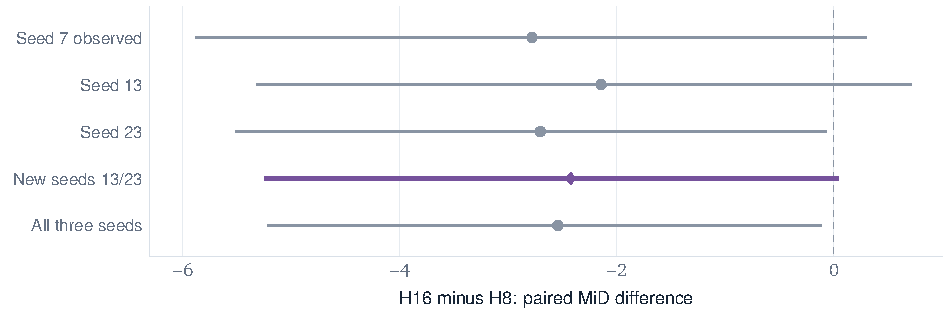
\includegraphics[width=0.98\linewidth]{figures/rev_h16.pdf}
\caption{Paired H16-minus-H8 MiD differences for three head seeds on OLD\_DEV.}
\label{fig:middle-h16}
\end{figure}

The full expert/context model outperformed every registered reduction. FULL-C0 scored 121.4 MiD, versus 127.8 for A5-only, 126.7 for C2F-only, and 124.7 for A5 plus PAIR. Unordered aggregation with age reached 122.4; removing explicit time gave 123.7. Each reduction failed the accuracy screen or its small-excess-error bound. The experts themselves can encode temporal information, so this comparison does not isolate recurrence as the source of the gain. \evidence{M_SIMPLEX}

The analytic EWMA/transport control lost to H8 on every sequence, scoring 155.4 versus 121.6 MiD; the hierarchical interval for the 33.8-point difference was $[17.1,51.0]$. WIDE averaged 119.0 across three head seeds, but its intervals against both H8 and H16 crossed zero. It was not promoted. \evidence{M_EWMA,M_WIDE}

\subsection{Capacity and teacher-feature coverage}

Stage70--76 and the V11 capacity extension planned direct, pairwise-predictive, trajectory, and temporal-permutation comparisons at approximately 2M, 4M, and 8M parameters. The 4M trajectory model was primary. The proposed 30,000-query set covered 27 sequences; extra timestamps increased density, not the number of independent acquisitions.

The V11 audit found teacher features for 4,775 historical tokens and none for the other 25,225. Matching token IDs also left ROI construction, RGB preprocessing, and teacher provenance unresolved. \evidence{M_CAPACITY_PROTOCOL,M_CAPACITY_AUDIT}

Stage70 ended with both completed and unfinished endpoints. The partial record supplies no capacity ranking and no evidence that unlabeled JEPA pretraining improved SIMPLEX-T. \evidence{M_STAGE70_LEDGER}

\section{Transfer, output stability, and runtime}
\label{sec:transfer-context}

\subsection{Development, training, and transfer populations}

The transfer studies answer different questions from OLD\_DEV and TRAIN40. OLD\_DEV had already guided development, and TRAIN40 includes fitted examples. EvTTC and Forward Collision Warning Data (FCWD) instead evaluate frozen models with dataset-specific adapters. FCWD contains three driving sequences with paired events, frames, and LiDAR-derived TTC \citep{eventaided}. The expanded EvTTC set adds timestamps to the same 32 sequences rather than a new holdout.

The earlier H8/TRAIN40 route predates the final refit in Section~\ref{sec:train40}. A5 and C2F each received 49,932 updates, the pair head 6,840, and each of three H8 heads 2,500. Its 88,744 training predictions diagnose fit but cannot estimate unseen-scene performance. Inference used events, while training also used an RGB teacher and geometric supervision. \evidence{M_SCIENCE_AUDIT}

The initial EvTTC evaluation had 946 valid targets among 1,024 queries from 32 sequences; the expansion had 3,640 among 3,947. FCWD contributed 597 eligible targets among 630 queries from three previously exposed sequences. We left rows without ground truth unscored, and all reported methods returned finite predictions on the eligible rows. Full RGB/event Garl was omitted from FCWD because the RGB-to-event mapping had not been verified. \evidence{M_V12_EVTTC_946,M_V12_EVTTC_3640,M_V12_FCWD_597}

\subsection{Input and output conditions}

H8 used retrospective event history and supplied oracle ROI metadata. Garl event-only used its native pair of event windows, while Garl full added RGB. The systems differed in context and input construction. EvTTC projected RGB to events with calibrated rotation but no depth-dependent parallax correction. These transfer adapters do not reproduce the published benchmark protocol.

We corrected RGB synchronization before running full Garl. Selected images had to lie within 1\,ms of each event endpoint and about 100\,ms apart; the largest admitted offset was 453\,$\mu$s. The runner strictly loaded the released checkpoint and upstream normalization. Because we designed the RGB extension after inspecting event-only results, this comparison remains exploratory even though the weights stayed frozen. \evidence{M_TRANSFER_REPORT}

H8 bounds TTC at $\pm60$ seconds. Garl keeps its native scale-ratio division, which emits very large finite values when the estimated scales nearly match. We retained those predictions in the full-population metrics.

\subsection{Transfer results and metric-dependent rankings}

% Generated by research/middle_tables.py; do not edit numeric values.
\begin{table}[tbp]
\centering\small
\caption{Frozen H8 and Garl models evaluated on EvTTC and FCWD.}
\label{tab:middle-transfer}
\setlength{\tabcolsep}{5pt}
\begin{tabular}{lrrrr}
\toprule
Method & MAE (s) & Median AE (s) & RMSE (s) & RTE (\%) \\
\midrule
\multicolumn{5}{l}{\textbf{EvTTC: 946 eligible / 1,024 queries; 32 sequences}} \\
H8 / head 7 & 1.321 & 0.766 & 3.027 & 62.35 \\
H8 / head 13 & 1.353 & 0.731 & 3.206 & 62.92 \\
H8 / head 23 & 1.409 & 0.738 & 3.392 & 68.87 \\
Garl event & 8.048 & 0.997 & 159.247 & 293.47 \\
Garl RGB + event & 1.868 & 0.692 & 7.875 & 76.77 \\
\midrule
\multicolumn{5}{l}{\textbf{EvTTC expanded: 3,640 / 3,947; same 32 sequences}} \\
H8 / head 7 & 1.361 & 0.722 & 3.475 & 53.70 \\
H8 / head 13 & 1.395 & 0.699 & 3.618 & 54.52 \\
H8 / head 23 & 1.456 & 0.702 & 4.003 & 59.15 \\
Garl event & 4.560 & 0.958 & 83.896 & 161.12 \\
Garl RGB + event & 94.510 & 0.661 & 5561.622 & 5180.18 \\
\midrule
\multicolumn{5}{l}{\textbf{FCWD: 597 / 630; three sequences}} \\
H8 / head 7 & 1.778 & 0.675 & 3.588 & 30.20 \\
H8 / head 13 & 1.597 & 0.580 & 3.258 & 27.41 \\
H8 / head 23 & 1.569 & 0.598 & 3.109 & 27.48 \\
Garl event & 2.146 & 0.602 & 5.072 & 26.89 \\
\bottomrule
\end{tabular}
\par\vspace{4pt}
\begin{minipage}{0.98\linewidth}\footnotesize Scores use queries with valid TTC targets; prediction coverage is 100\% on these queries. H8 bounds TTC at $\pm60$\,s, while Garl retains its native signed outputs. The FCWD comparison uses event-only inputs. \evidence{M_V12_EVTTC_946,M_V12_EVTTC_3640,M_V12_FCWD_597}\end{minipage}
\end{table}


H8 had the lowest mean error on the first 946 EvTTC targets: its three heads reached 1.32--1.41 seconds MAE, versus 8.05 for Garl event-only and 1.87 for Garl full. Garl full had the best median, 0.69 seconds versus 0.73--0.77 for H8. \evidence{M_V12_EVTTC_946}

The 3,640-target expansion showed the same split. H8 achieved 1.36--1.46 seconds MAE, Garl event-only 4.56, and Garl full 94.51. Yet Garl full retained the best median at 0.66 seconds, ahead of H8's 0.70--0.72. Rare near-singular scale ratios drove Garl full's mean, so native-output and matched-clipping results remain separate. \evidence{M_V12_EVTTC_3640}

On FCWD, H8 led in MAE at 1.57--1.78 seconds versus 2.15 for Garl event-only. Garl led in mean relative TTC error at 26.9\%, compared with 27.4--30.2\% for H8. These rankings weight the TTC distribution differently, and only three sequences were available for clustered uncertainty. \evidence{M_V12_FCWD_597}

\subsection{Head and full-route runtime}

% Generated by research/middle_tables.py; do not edit numeric values.
\begin{table}[tbp]
\centering\small
\caption{Head-only and full-pipeline runtime.}
\label{tab:middle-cost}
\setlength{\tabcolsep}{5pt}
\begin{tabular}{l@{\hspace{12pt}}r@{\hspace{12pt}}r@{\hspace{12pt}}r@{\hspace{12pt}}r}
\toprule
Model & MiD & Head p95 (ms) & Route 1 p95 (s) & Route 2 p95 (s) \\
\midrule
H1\_SEED7 & 132.832 & 9.28 & 2.944 & 2.902 \\
H8\_SEED7 & 121.646 & 19.47 & 9.349 & 8.479 \\
H16\_SEED7 & 118.866 & 31.45 & 13.201 & 15.304 \\
FULL\_C0 & 121.405 & 21.07 & 8.477 & 9.337 \\
A5\_ONLY\_C0 & 127.785 & 21.42 & 7.928 & 7.471 \\
C2F\_ONLY\_C0 & 126.705 & 19.28 & 8.185 & 8.256 \\
A5\_PAIR\_C0 & 124.669 & 19.83 & 7.086 & 7.502 \\
SET\_AGE\_C0 & 122.443 & 10.00 & 7.628 & 8.303 \\
SET\_NOTIME\_C0 & 123.687 & 9.91 & 7.727 & 7.967 \\
\bottomrule
\end{tabular}
\par\vspace{4pt}
\begin{minipage}{0.98\linewidth}\footnotesize Head: median of three blockwise p95 values, CPU FP32, prepared inputs, 500 measurements per block. Route: p95 on 64 TRAIN queries with supplied ROI, shared GPU, and resident producers. Accuracy uses OLD\_DEV seed 7, nine sequences and three folds. \evidence{M_HEAD_COST,M_ROUTE_COST}\end{minipage}
\end{table}


Prepared-input CPU profiling measured three rotated-order blocks of 500 batch-one calls per head. Median blockwise p95 was 9.28\,ms for H1, 19.47\,ms for H8, and 31.45\,ms for H16. The timer covered canonical TTC emission, but not event reading, ROI construction, expert inference, detection, or tracking. \evidence{M_HEAD_COST}

The shared-GPU route was much slower than the isolated heads. Across 1,728 supplied-ROI requests from 64 TRAIN queries, H8 p95 was 9.35 and 8.48 seconds in two warm blocks; H16 reached 13.20 and 15.30 seconds. The application reopened HDF5 inputs between cold measurements, while the operating system could retain cached pages. \evidence{M_ROUTE_COST}

ROI/voxel reading and preparation consumed 85.5\% of H8's measured time and 90.4\% of H16's in the second warm block. We focused V12 on preparation, bounded caching, and transfer scheduling rather than head speed alone. \evidence{M_ROUTE_REPORT}

CUDA graphs reduced recorded A5 launches from 5,877 to 1,270 while preserving the tested outputs, losses, RNG state, and gradients. A later window measured 41.78 versus 32.89 updates/min, but host load and data wait also changed, so the run did not isolate graph speedup. Adaptive caching reached 26.31 updates/min against a 36.75 reference and failed its throughput test. \evidence{M_ENGINEERING}
